\documentclass[hidelinks, 12pt]{article}
\usepackage{amsmath, amsthm, amsfonts}
\usepackage[top=1in, bottom=1in, left=1in, right=1in]{geometry}
\usepackage{setspace}
\usepackage{sectsty}
\usepackage{lipsum}
\usepackage{hyperref}
\usepackage{indentfirst}
\usepackage{tikz}
\usetikzlibrary{automata,topaths}
\usepackage{graphicx}
\graphicspath{{images/}}
\usepackage{caption}
\usepackage{subcaption}
\usepackage{pgfplots}
\pgfplotsset{compat=1.6}
\usepackage{float}
\usepackage[normalem]{ulem}
\usepackage{color}
\usepackage{framed}
\usepackage{wrapfig}
% \usepackage[%
%     font={small,sf},
%     labelfont=bf,
%     format=hang,
%     format=plain,
%     margin=0pt,
%     width=0.8\textwidth,
% ]{caption}
% \usepackage[list=true]{subcaption}

\usepackage[square,numbers]{natbib}
\bibliographystyle{unsrtnat}

\definecolor{codebg}{rgb}{0.95,0.95,0.95}
\doublespacing

\begin{document}
\title{\vspace{-1in}Effects of Sitka Spruce succession on soil nutrients near anadromous fish bearing watersheds.}
\author{Will Dumm}
\maketitle
\hrulefill
% \tableofcontents
% \hrulefill
\vspace{.2in}

% \setlength{\columnsep}{10pt}
\begin{wrapfigure}{r}{3.4in}
    \vspace{-10pt}
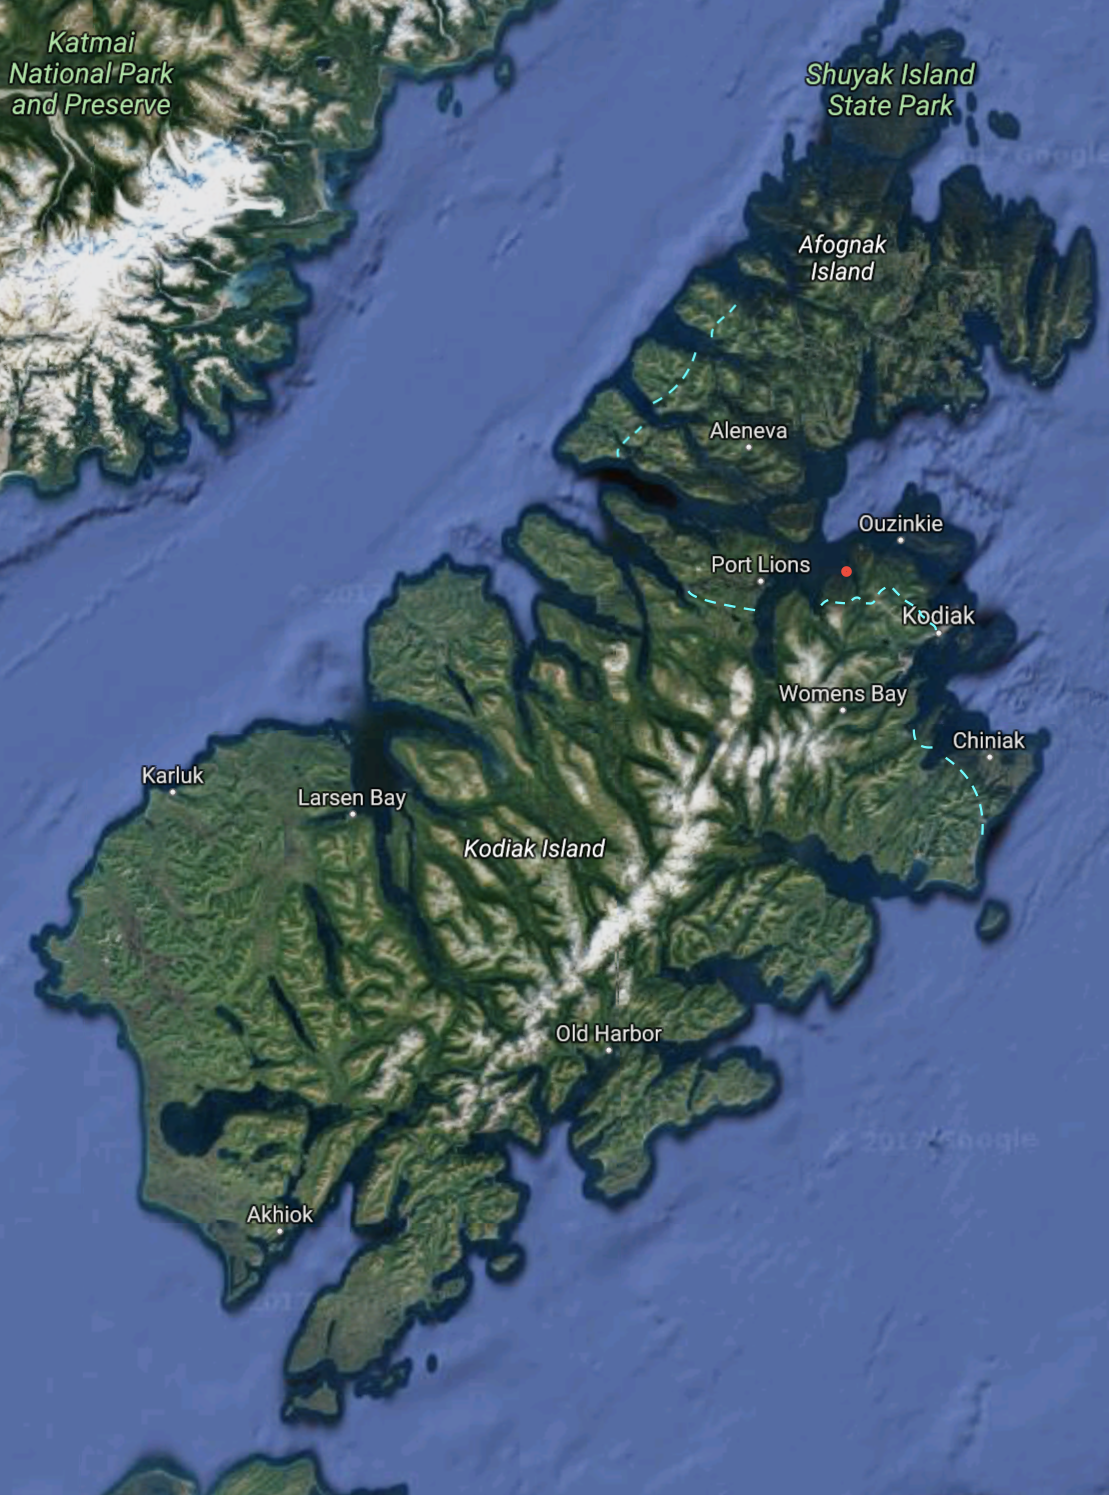
\includegraphics[width=3.5in]{Kodiak.png}
\caption{Sitka spruce colonization of Kodiak Island. Southward advancing front of spruce forest is approximated by the dotted line, with site location marked in red.}
\label{fig:Kodiak}
\vspace{-10pt}
\end{wrapfigure}

12000 years ago, the last major glacial advance in Southcentral Alaska, the Akalura advance, began to recede \cite{NelsonPollenRecord}. At the time, ice covered nearly all of Kodiak Archipelago and the neighboring Alaska Peninsula, as well as coastal Southcentral and Southeast Alaska. Following the retreat of the ice sheet, coastal forest began to advance northwest along the coast from forests in Washington and British Colombia. This advance continues today, with forests of Sitka spruce, which took root on the northern end of the Kodiak Archipelago as recently as 800 years ago, now spreading southwest across the northern tip of Kodiak Island. In areas newly colonized by spruce forest, soil structure and chemistry are likely to change.



Kodiak Island is home to hundreds of lakes and rivers which serve as important habitat for Pacific salmon. As landlocked fry, salmon rely heavily on accumulated marine-derived nutrients transported to lake sediment by previous spawning runs. However, they are also sensitive to runoff from surrounding soil \cite{Naiman2002, ChalonerMarineNitrogen}. As spruce forest becomes the dominant land cover in the region, I would like to understand the effects of associated changes in nutrient storage, availability, and runoff on salmon habitat.

\begin{wrapfigure}{r}{3.5in}
    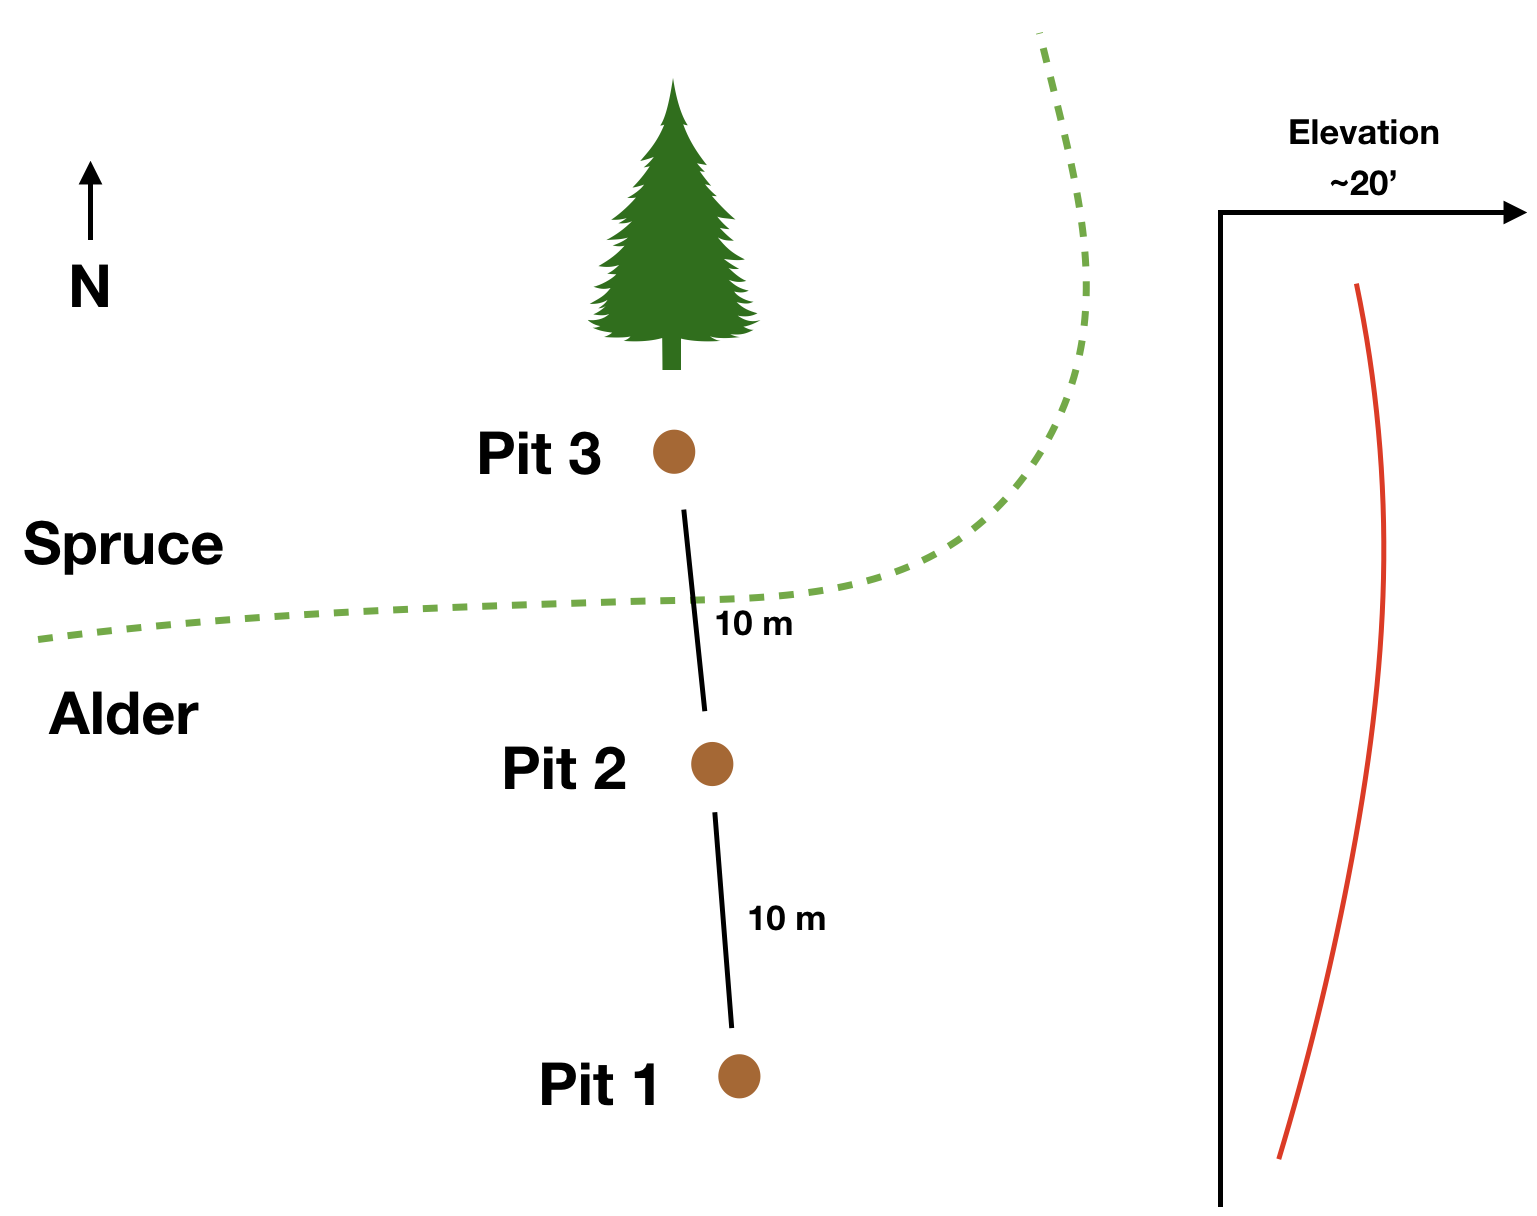
\includegraphics[width=3.5in]{Sitediagram.png}
    \caption{Site Layout}
    \label{fig:sitediagram}
\end{wrapfigure}

This project will focus on changes in soil nitrogen content in soil newly colonized by spruce forest. We will test samples from three soil pits on Anton Larsen Island, arranged across a boundary between well-established (greater than 50 year-old) spruce forest and an older Sitka alder forest. Site location is shown in Figure~\ref{fig:Kodiak}, and pit arrangement is shown in Figure~\ref{fig:sitediagram}.

Sitka alder is a nitrogen fixing species, while Sitka spruce is not. In many areas, soils are also fertilized by salmon carcasses transported from nearby salmon-bearing streams by predators. However, Anton Larsen Island is more than two miles by land from the nearest salmon stream, so vegetation is likely the dominant source of soil nitrogen. We expect to observe similar marine-derived soil nitrogen content in the adjacent spruce and alder forest habitats, but lower atmospheric nitrogen content in soils colonized by spruce.


\begin{figure}[H]
    \begin{minipage}{2in}
        \centering
    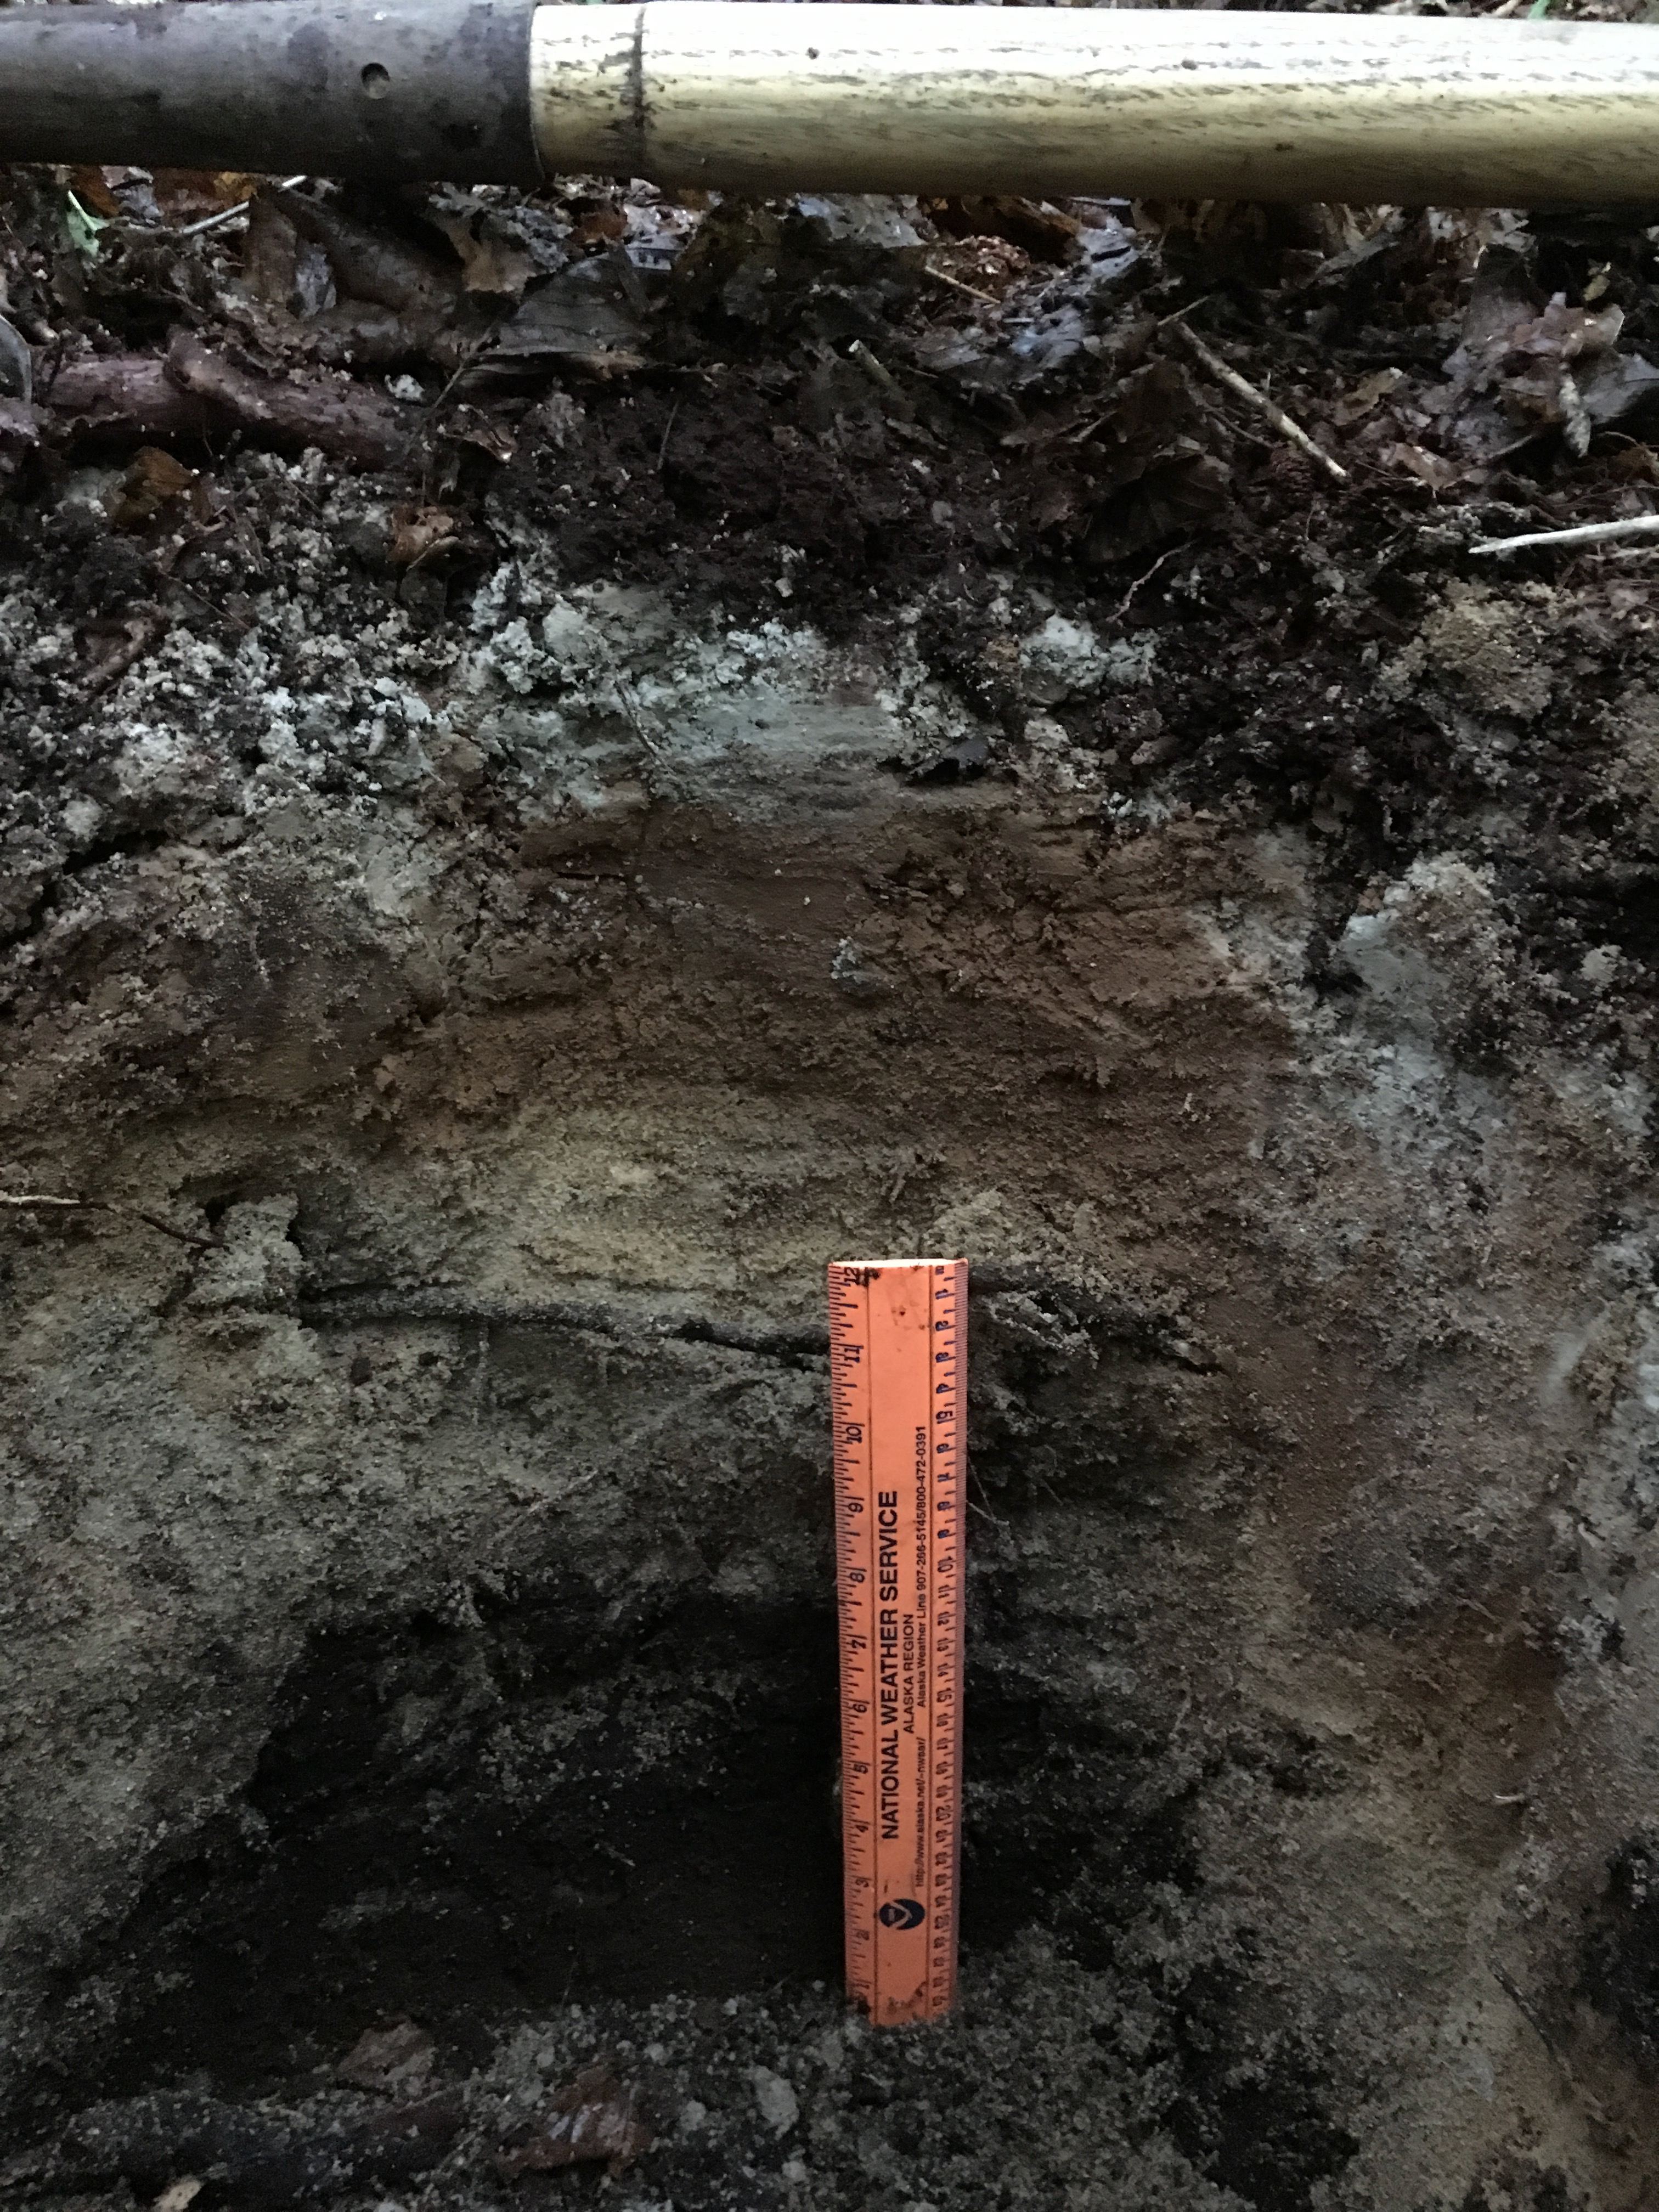
\includegraphics[width=2in]{pit1.jpg}
    \subcaption{Pit 1}
    \end{minipage}\hfill
    \begin{minipage}{2in}
        \centering
    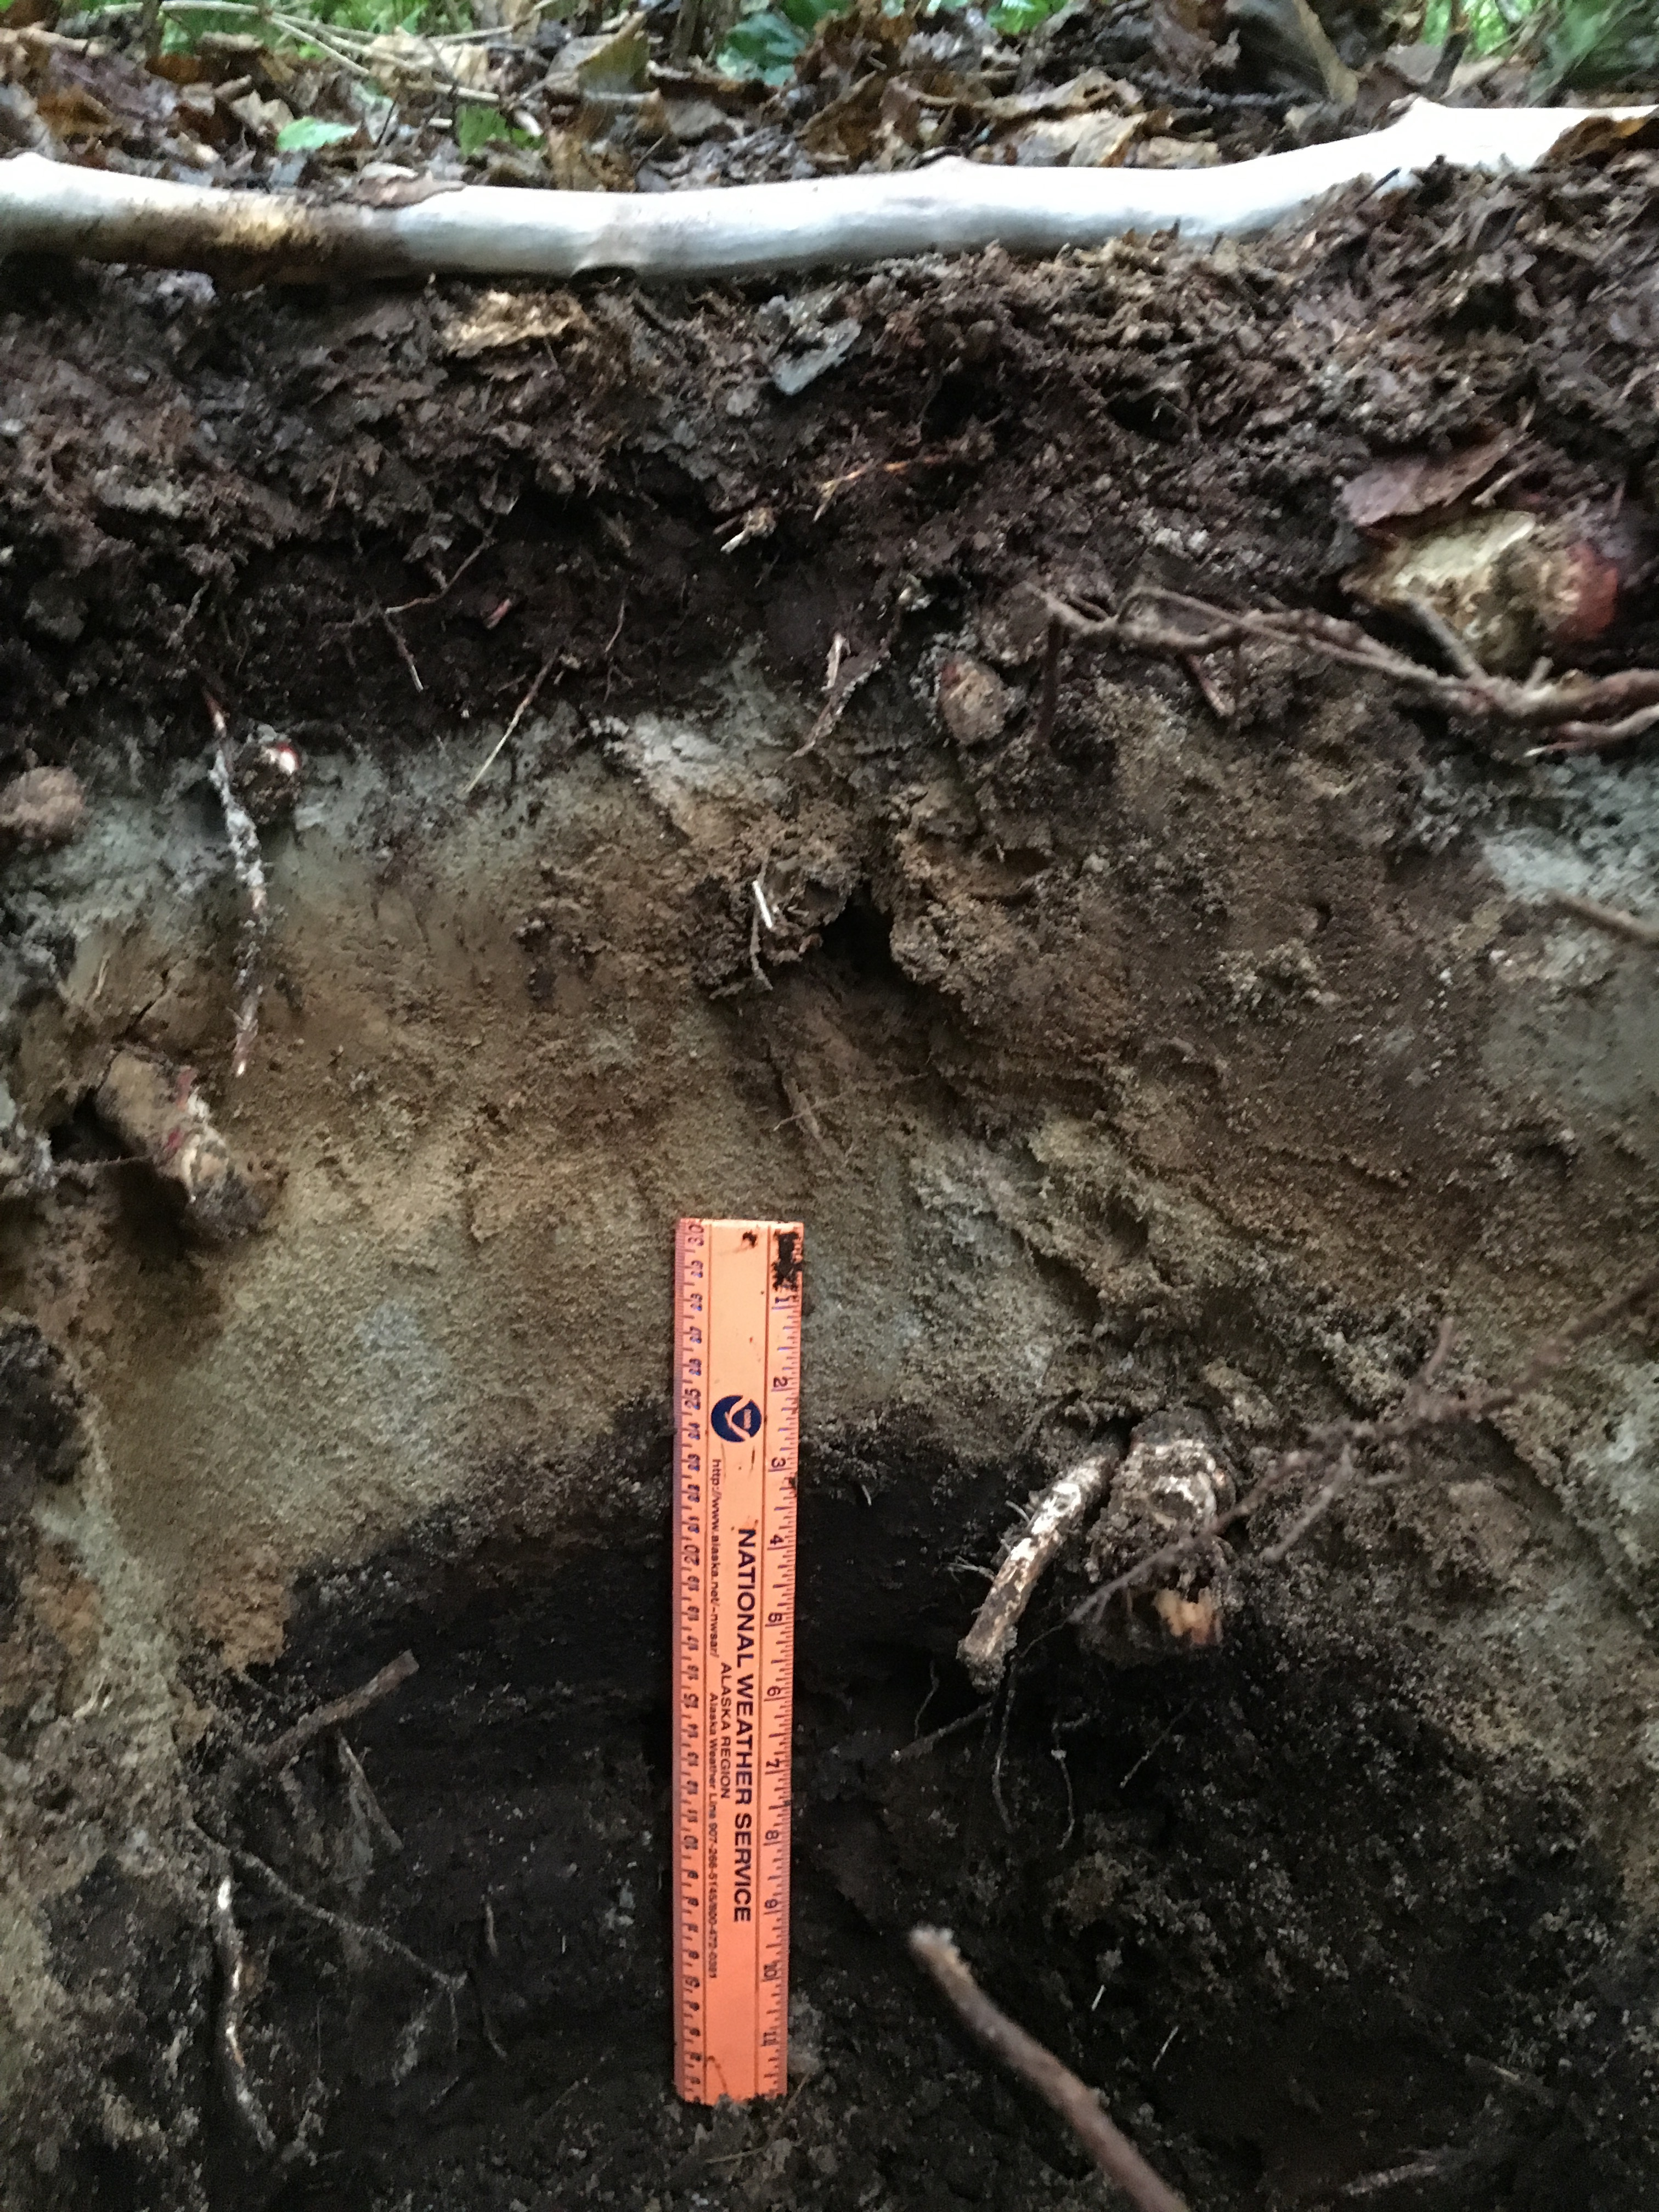
\includegraphics[width=2in]{pit2.JPG}
    \subcaption{Pit 2}
    \end{minipage}\hfill
    \begin{minipage}{2in}
        \centering
    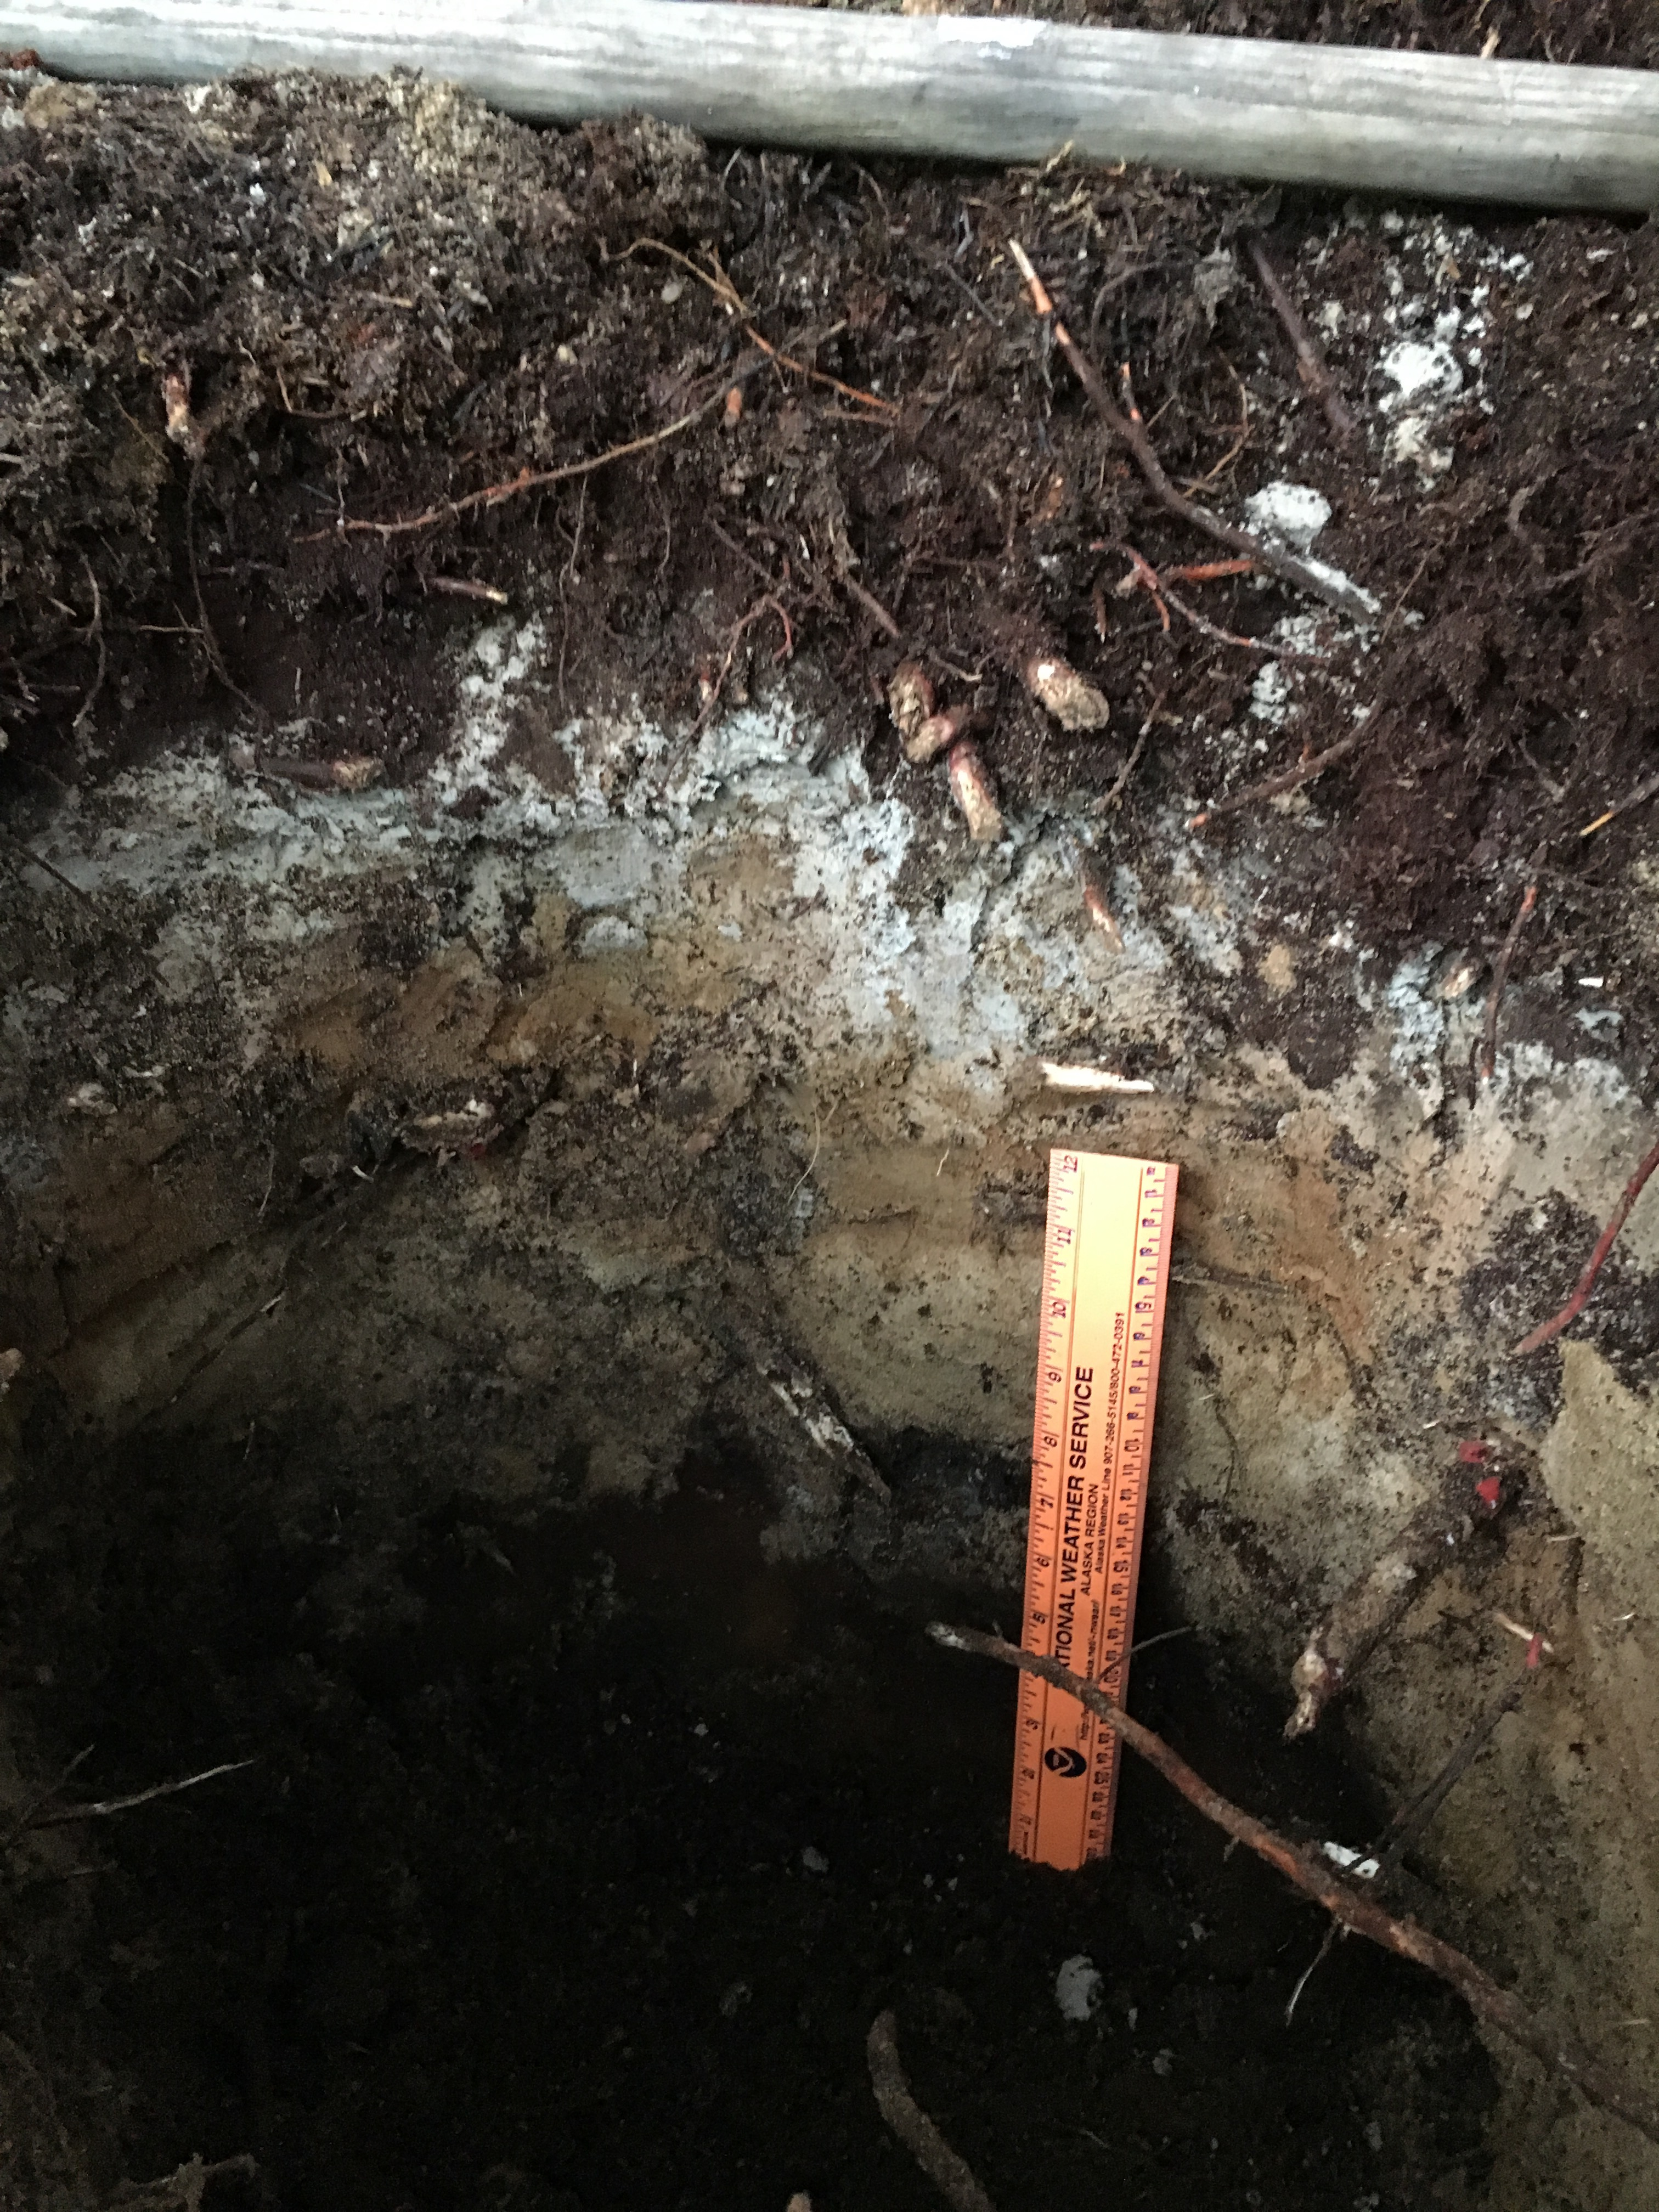
\includegraphics[width=2in]{pit3.JPG}
    \subcaption{Pit 3}
    \end{minipage}

    \caption{Soil Profiles}
    \label{fig:pits}
\end{figure}

Soil profiles in all three pits are shown in Figure~\ref{fig:pits}. The profiles consist of approximately the following horizons:

\begin{center}
 \begin{tabular}{||c | c | c||}
 \hline
 Horizon & Depth & Composition \\ [0.5ex]
 \hline\hline
 Oi & 0-1" & Organic matter \\
 \hline
 Oe & 1-3" & Decomposed Organic Matter\\
 \hline
 C1 & 3-7" & Volcanic Ash \\
 \hline
 C2 & 7-9" & Volcanic Ash \\
 \hline
 C3 & 9-12" & Volcanic Ash\\
 \hline
 Bb & 12-20" & Silt loam with gravel \\
 \hline
 Cb & $>$20" & gravel/bedrock \\ [1ex]
 \hline
\end{tabular}
\end{center}

A thick layer of up to a foot of volcanic ash characterizes soils across much of the archipelago. This ash was deposited following the Katmai-Novarupta eruption of 1912 \cite{hildreth2012novarupta}. At the location which we are considering, spruce colonization began strictly after the eruption; horizons beneath the volcanic ash layer formed completely uninfluenced by the presence of Sitka spruce. The degree to which the transition to spruce forest effects nutrients in these capped horizons will give an indication of the rate of nutrient leaching and runoff.






\newpage

\bibliography{references}

\end{document}
